\begin{center}
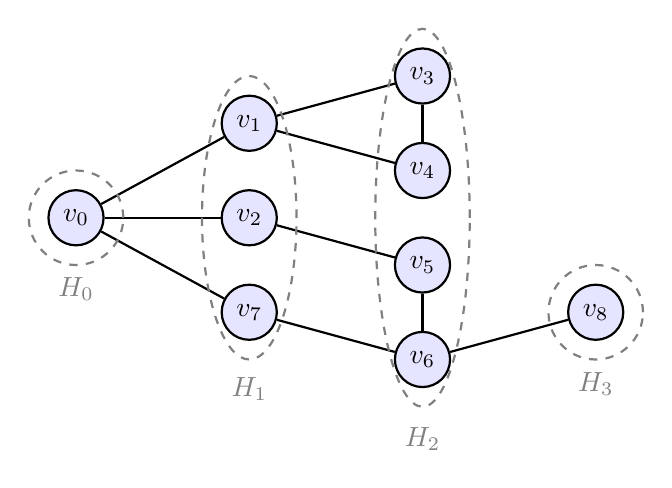
\begin{tikzpicture}[
  vnode/.style={circle, draw, minimum size=7mm, inner sep=0pt, fill=blue!10},
  thick
]
  % Nodes
  \node[vnode] (v0) at (0, 0) {$v_0$};
  
  \node[vnode] (v1) at (2.2, 1.2) {$v_1$};
  \node[vnode] (v2) at (2.2, 0) {$v_2$};
  \node[vnode] (v7) at (2.2, -1.2) {$v_7$};
  
  \node[vnode] (v3) at (4.4, 1.8) {$v_3$};
  \node[vnode] (v4) at (4.4, 0.6) {$v_4$};
  \node[vnode] (v5) at (4.4, -0.6) {$v_5$};
  \node[vnode] (v6) at (4.4, -1.8) {$v_6$};
  
  \node[vnode] (v8) at (6.6, -1.2) {$v_8$};
  
  % Edges
  \draw (v0) -- (v1);
  \draw (v0) -- (v2);
  \draw (v0) -- (v7);
  
  \draw (v1) -- (v3);
  \draw (v1) -- (v4);
  \draw (v2) -- (v5);
  \draw (v7) -- (v6);
  
  \draw (v6) -- (v8);
  
  \draw (v3) -- (v4);
  \draw (v5) -- (v6);
  
  % Elipsy pro hladiny
  \draw[gray, dashed] (0, 0) circle [x radius=0.6, y radius=0.6] node[below=18pt] {$H_0$};
  \draw[gray, dashed] (2.2, 0) ellipse [x radius=0.6, y radius=1.8] node[below=54pt] {$H_1$};
  \draw[gray, dashed] (4.4, 0) ellipse [x radius=0.6, y radius=2.4] node[below=72pt] {$H_2$};
  \draw[gray, dashed] (6.6, -1.2) circle [x radius=0.6, y radius=0.6] node[below=18pt] {$H_3$};
\end{tikzpicture}
\par\medskip
\textit{Obrázek 2.1: Rozklad grafu na hladiny $H_0, H_1, H_2, H_3$ podle vzdálenosti od $v_0$.}
\end{center}